%!TEX root = main.tex

\section{Empirical Methodology}\label{methodology}

%We employed exploratory interviews with software practitioners and surveys of practitioners to validate our findings.

To understand the merge conflict resolution processes employed by software developers, we used mixed methods consisting of interviews to gather qualitative insights and surveys to provide quantitative triangulations into the broader context of merge conflicts in software development.
Mixed methods allow us to identify perspectives and themes from both individual and population-wide samples to strengthen the validity of both, as per guidelines from \mbox{Easterbrook et al.}~\cite{easterbrook2008selecting}.

In this study, we were particularly interested in understanding the processes that software developers have developed or adopted in order to successfully resolve merge conflicts.
Processes are developed to address common problems in teams and organizations and identifying the problems is an essential element to process improvement~\cite{beecham2003software}.
To analyze the processes, we first sought to understand the difficulties that inhibit developers from successfully resolving merge conflicts.

We conducted exploratory interviews with software developers to create a taxonomy of barriers, constraints, and concerns experienced when encountering merge conflicts (\textit{Interviews}).
We then triangulated our results by conducting a survey on the broader developer community, using the vocabulary generated from the interviews to create the survey questions related to how they approach merge conflicts (\textit{Perceptions Survey}).
Based upon these initial studies, we additionally developed a targeted survey to understand how developers monitor for merge conflicts, employ strategies for resolving them, and evaluate whether their strategies are successful (\textit{Processes Survey}).

\subsection{Exploratory Interviews}\label{interviews}

Semi-structured interviews provide qualitative data collection through open-ended questions that elicit interviewee's thoughts and opinions about a particular topic.
The resulting data includes themes and terminology from the perspective of the interviewee, as opposed to the interviewer, and provides a context for further quantitative inquiry~\cite{easterbrook2008selecting}.

We conducted semi-structured interviews with software developers to understand their concerns when facing merge conflicts and the factors that impact merge conflict difficulty.
We selected interview participants from top contributors to open-source projects, and from industry contacts using snowball sampling~\cite{goodman1961snowball} to reach a larger sample size.
Each participant was asked to identify additional practitioners for recruitment to our study.

We interviewed ten software developers from seven different organizations spanning six different industries.
The participants primarily worked on open-source projects (eight of the ten participants), and focused on projects that ranged in size from less than five active contributors to more than 1700 contributors (for a 12-month period).
Table~\ref{interview_demographics} provides additional demographics data, including software development experience, role, industry, project size, and whether the participant primarily focused on open- or closed-source software development.

\begin{table}[!htbp]
\renewcommand{\arraystretch}{1.3}
\caption{Interview Participant Demographics}
\label{interview_demographics}
\centering
\begin{tabularx}{\textwidth}{@{}llllrr@{}}
\toprule
	\parnoteclear % tabularx will otherwise add each note thrice
	\textbf{Par.}\parnote{Par. = Interview Participant} & \textbf{Exp.}\parnote{Exp. = Years of Software Development Experience} & \textbf{Role} & \textbf{Industry} & \textbf{Source}\parnote{Source = Source Code Licensing in primary project} & \textbf{\mbox{Contrib.}}\parnote{Contrib. = Approximate number of individual contributors in primary project (between March 2016-March 2017)}\\
\midrule
	P1 & 18 yrs. & Sr. \mbox{Software} \mbox{Developer} & Semiconductor Mfr. & Open & 1700\\
	P2 & 6 yrs. & Software \mbox{Engineer} & Semiconductor Mfr. & Open & 1700\\
	P3 & 3 yrs. & Software \mbox{Engineer} & Semiconductor Mfr. & Open & 1700\\
	P4 & 10 yrs. & Software \mbox{Developer} & Academia & Open & \textless10\\
	P5 & 3 yrs. & Infrastructure \mbox{Engineer} & Healthcare Software & Closed & \textless10\\
	P6 & 5 yrs. & Software \mbox{Developer} & Healthcare Software & Closed & \textless10\\
	P7 & 5 yrs. & Software \mbox{Engineer} & Business Software & Open & 200\\
	P8 & 25 yrs. & Director & Academia & Open & 600\\
	P9 & 8 yrs. & Software \mbox{Developer} & IT Services & Open & 600\\
	P10 & 2 yrs. & Software \mbox{Developer} & Sports Software & Open & \textless5\\
\bottomrule
\end{tabularx}
\parnotes
\end{table}

Additional details regarding the study format, questions, and analysis of the exploratory interviews is presented elsewhere~\cite{mckee2017software}.

\subsection{Perceptions Survey}\label{perceptions_survey}

Surveys are commonly used to for mapping the state of practice, establishing baselines for investigating research topics, and gathering opinions regarding software engineering technologies and practices~\cite{deMello2016survey}.
We conducted a 50-question \textit{Perspectives Survey} of software developers in order to examine the barriers, constraints, and concerns experienced when encountering merge conflicts.
We developed questions to confirm, extend, and broaden the results from the interviews and provide context for the questions in our \textit{Processes Survey}.

\renewcommand*{\thefootnote}{\arabic{footnote}}
\setcounter{footnote}{0}
We recruited \textit{Perceptions Survey} participants from contributor lists on popular open-source repositories on GitHub, advertised on social networking sites (Facebook and Reddit), and by directly contacting software developers via email. 
Due to the nature of social media and mailing lists, we cannot compute a response rate. 
However, our participants spanned different organization structures and geographical locations, giving us generalizability of results.
The survey was conducted online and anonymity was guaranteed in order to elicit honest responses from participants.
The survey was available for 56 days and we received 162 survey responses, but individual parts of the survey have varying response rates and are reported where appropriate in Section~\ref{results}. 

Survey participants were given six different software roles to select, and in many cases, participants considered themselves to be fulfilling multiple roles. 
Table~\ref{survey_roles} provides a pairwise breakdown of participants' role selections, with a majority of respondents considering themselves to be \textit{Software Engineer/Developer} (95.1\% overall).
Survey participants indicated a median software development experience of 6-10 years (36.4\% overall), and worked on project sizes ranging from 2 to more than 51 developers (the median was 2-5 developers, constituting 48.8\% of all responses).

\begin{table}[!htbp]
%\renewcommand{\arraystretch}{1.3}
\caption{Perceptions Survey Participant Roles\textsuperscript{i}}
\label{survey_roles}
\centering
\begin{tabularx}{\textwidth}{@{}r|*{10}{C}c@{}}
\toprule
\addlinespace[4.5em]
	& \begin{rotate}{30} Soft. Developers \end{rotate} 
	& \begin{rotate}{30} Sys. Architects \end{rotate} 
	& \begin{rotate}{30} DevOps \end{rotate} 
	& \begin{rotate}{30} Project Managers \end{rotate}
	& \begin{rotate}{30} Project Maintainers \end{rotate}
	& \begin{rotate}{30} Sys. Admins \end{rotate}
	& \begin{rotate}{30} Other \end{rotate}\\
\midrule
	Software Developers & 154 & & & & & & \\
	System Architects & 53 & 54 & & & & & \\
	DevOps & 51 & 34 & 53 & & & & \\
	Project Managers & 44 & 29 & 20 & 44 & & & \\
	Project Maintainers & 39 & 21 & 24 & 22 & 40 & & \\
	Systems Administrators & 22 & 16 & 15 & 14 & 12 & 23 & \\
	Other & 8 & 4 & 4 & 3 & 1 & 2 & 11 \\
\bottomrule
	\multicolumn{8}{c}{\noindent\parbox[t]{11.7cm}{\vspace{0.7em}\textsuperscript{i}\hspace{0.2em}\textit{Perceptions Survey} respondents were allowed to select multiple roles. Each entry represents the number of respondents that selected both of the roles indicated for the column and row. 62 out of 162 respondents (38\%) selected three or more roles.}}
\end{tabularx}
\end{table}

The \textit{Perceptions Survey} was divided into four categories, with each category containing 5-7 questions (see \cite{companion_site} for questions).
First, we elicited background information about demographics, roles, and experience.
Second, we asked questions related to difficulties that developers experience when encountering merge conflicts.
Third, we asked questions related to conflict resolution and the factors that affect developers.
Finally we asked questions about the tools and tool features that developers use when working with merge conflicts.
Questions were presented either as 5-point Likert-type scales (with no pre-selected answers) or open-ended text forms to gather additional insights.

\subsection{Processes Survey}\label{processes_survey}

Based on the results from the \textit{Exploratory Survey} (Section~\ref{interviews}) and the \textit{Perceptions Survey} (Section~\ref{perceptions_survey}), we observed that developers have created or adopted processes for maintaining awareness, planning solutions, and evaluating their resolutions to merge conflicts.
To understand the prevalence and variety of these merge conflict processes, we conducted an additional 15-question \textit{Processes Survey} among software developers.

We recruited survey participants using similar methods as the \textit{Perceptions Survey} to allow for comparisons and triangulation of the results.
The survey was conducted online and anonymity was guaranteed.
We advertised on social networking sites (Twitter and Reddit), and through emails to industry contacts and interview participants to locate additional software developers using snowball sampling.
The survey was available for 38 days and we received 113 survey responses, however, 11 responses were removed due to being incomplete and abandoned (not completed after one week); results for 102 survey responses are presented in Section~\ref{results}.

Survey participants were assumed to be software developers in some capacity, but primary roles within individual organizations can differ throughout the industry.
Participants were given seven different software roles to select, as well as an \texttt{Other:} field to provide additional roles not included in the pre-populated options.
Figure~\ref{processes_roles}

\begin{figure}[!htbp]
\centering
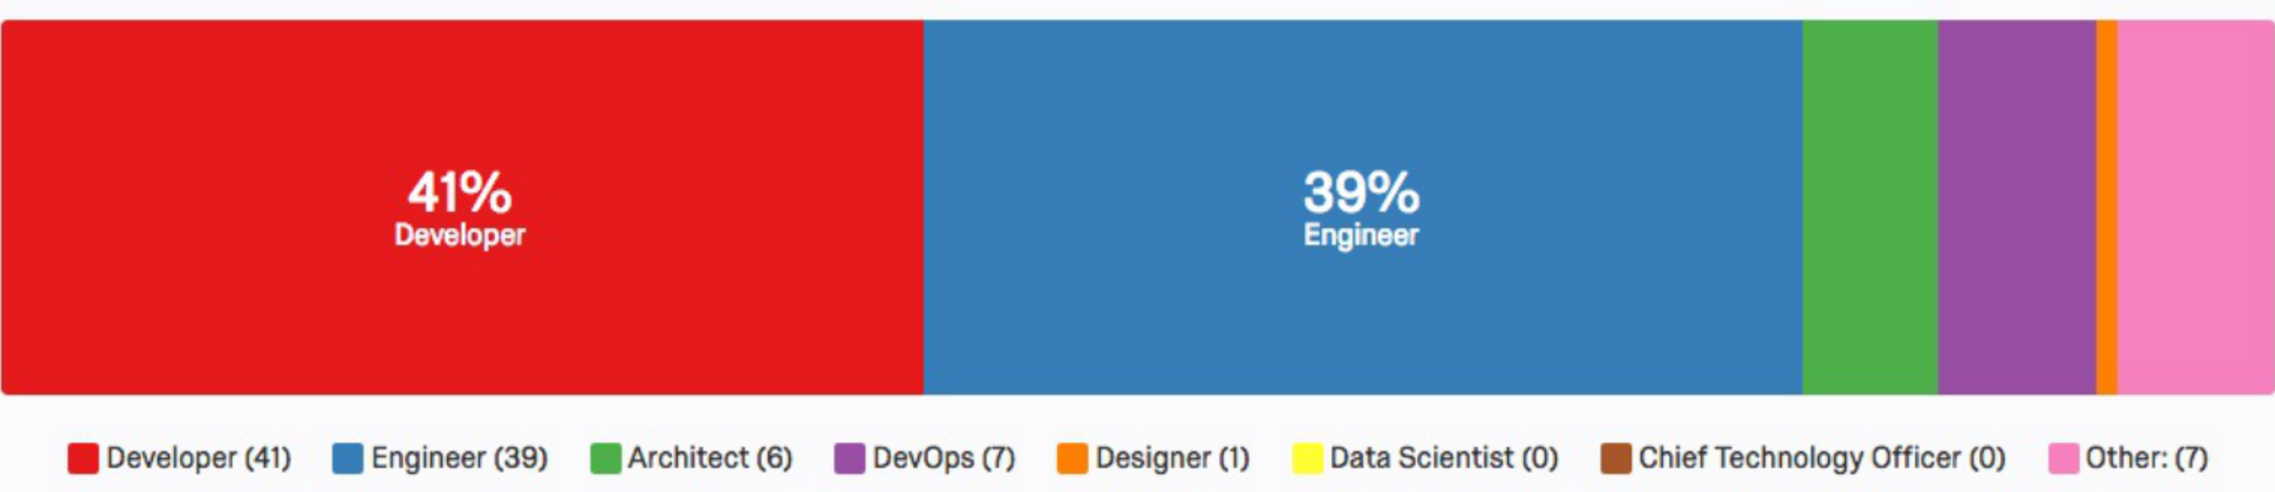
\includegraphics[width=0.98\textwidth,height=8em]{ProcessesParticipantRoles}
\caption{Participant role responses from \textit{Processes Survey}}
\label{processes_roles}
\end{figure}

%\subsection{Perceptions Survey}\label{perceptions_survey}
%
%We conducted a 50-question survey of software development practitioners in order to examine the themes and categories found in the interviews. We sought to understand which factors impact practitioners the most when they encounter and resolve merge conflicts.
%The survey was conducted online and anonymity was guaranteed in order to elicit honest responses from participants.
%We developed questions to confirm, extend, and broaden the results from the interviews.
%
%
%\renewcommand*{\thefootnote}{\arabic{footnote}}
%\setcounter{footnote}{0}
%We recruited survey participants from contributor lists on popular open-source repositories on GitHub\footnote{github.com}, advertised on social networking sites (Facebook\footnote{facebook.com} and Reddit\footnote{reddit.com}), and by directly contacting software practitioners via email. 
%Due to the nature of social media and mailing lists, we cannot compute a response rate. 
%However, our participants spanned different organization structures and geographical locations, giving us generalizability of results.
%The survey was available for 56 days and we received 162 survey responses, but individual parts of the survey have varying response rates and are reported where appropriate in Section~\ref{results}.
%
%%spanned six different software roles, ranging from system architects to system administrators (see Table~\ref{survey_roles}). 
%
%Survey participants were primarily male (91.9\% overall). 
%Participants were given six different software roles to select, and in many cases, participants considered themselves to be fulfilling multiple roles. 
%Table~\ref{survey_roles} provides a pairwise breakdown of participants' role selections, with a majority of respondents considering themselves to be \textit{Software Engineer/Developer} (95.1\% overall).
%Survey participants indicated a median software development experience of 6-10 years (36.4\% overall), and worked on project sizes ranging from 2 to more than 51 developers (the median was 2-5 developers, constituting 48.8\% of all responses).
%
%The survey was divided into four categories, with each category containing 5-7 questions (see \cite{companion_site} for questions).
%First, we elicited background information about demographics, roles, and experience.
%Second, we asked questions related to difficulties that practitioners experience when encountering merge conflicts.
%Third, we asked questions related to conflict resolution and the factors that affect practitioners.
%Finally we asked questions about the tools and tool features that practitioners use when working with merge conflicts.
%Questions were presented either as 5-point Likert-type scales (with no pre-selected answers) or open-ended text forms to gather additional insights.
%
%\Subsubsection{Analysis} We evaluated the distribution of survey answers for each Likert-type question by analyzing across demographic categories.
%Where answers differed across a demographic category, we note the difference and provide further discussion of these results in Section~\ref{results}.
%
%We used Likert-type questions to measure the extent to which participants agreed with a particular statement. This means that lower mean and median values indicate less agreement with the statement in a particular question.
%% As a result, a value of 1 and a value of 5 do not represent opposing opinions that we would see in a Likert scale that gives options from \textit{Strongly disagree} to \textit{Strongly agree}.
%We use this design to validate both the degree of agreement to the interview results, as well as the existence of individual factors.
%%This allowed us to verify interview results with larger-scale survey results.
